\documentclass{beamer}
\usepackage{amsmath, amssymb}
\usepackage{bm}
\usepackage{luatexja}
\usepackage{mathrsfs}              % 花文字
\usepackage{multirow}              % 表結合
\usepackage{float}                 % 図の位置制御
\usepackage{url}                   % URL表示
\usepackage{type1cm}               % フォント調整
\usepackage{here}                  % H位置指定
\usepackage{physics}               % 量子力学向け記法
\usepackage{graphicx}
\title{異なる一電子基底を使った二電子CI比較}
\subtitle{H軌道(非CF軌道)vsF軌道(SCF軌道)}
\author{藤原大地}
\date{2025年7月4日}
\setbeamertemplate{footline}[frame number]
\begin{document}

\frame{\titlepage}

% --- 1.1 試行関数 ---

  
\begin{frame}{目次}
  \begin{itemize}
    \item 第1章 理論(前回のおさらい)
    \item 第2章 プログラム概要
    \item 第3章 結果と考察
    \begin{itemize}
      \item 3.1 多電子波動関数の比較
      \item 3.2 エネルギーの$\omega$依存性
    \end{itemize}
  \end{itemize}
\end{frame}
  
% --- 1.1 試行関数 ---
\begin{frame}{第1章 理論}
\textbf{中間規格化}された多電子波動関数$\ket{\Phi_0}$を導入する
  \begin{align*}
  \ket{ \Phi_0} = \ket{\Psi_0}+ \sum_{a, r} c_a^r \ket{\Psi_a^r} + \sum_{a < b,\, r < s} c_{ab}^{rs} \ket{\Psi_{ab}^{rs}} + \cdots
  \end{align*}
  このとき、\textbf{Full CIエネルギー}$E_{Toal}$は\textbf{HFエネルギー}$E_0$と\textbf{相関エネルギー}$E_{\mathrm{corr}}$に分けられる:
  \begin{align*}
  E_{Total} &= E_0 + E_{\mathrm{corr}} 
  \end{align*}
  \textbf{HFエネルギー}:基底スレーターのみの多電子エネルギー
  \begin{align*}
  E_0 &= \mel{\Psi_0}{\mathscr{H}}{\Psi_0}
  \end{align*}
  \textbf{相関エネルギー}:電子相関に起因する負のエネルギー
  \begin{align*}
  (\mathscr{H} - E_0)\ket{\Phi_0} = E_{\mathrm{corr}} \ket{\Phi_0} 
  \end{align*}



\end{frame}
\begin{frame}{}
  \textbf{遷移エネルギー}はつぎの形で計算され
\begin{align*}
  H_ij = \mel{\Psi_i}{\mathscr{H}}{\Psi_{j}}
  \end{align*}

  次に二つの要請を満たすとき$H_{ij}=0$である
  \begin{itemize}
    \item ${\Psi_i}$と${\Psi_{j}}$で$Sz$固有値が保存されない
  \item ${\Psi_i}$と${\Psi_{j}}$で異なる違いが3個以上
  \end{itemize}


\end{frame}


\begin{frame}{第2章 プログラム概要}

  \begin{columns}
  % \column{0.5\textwidth} 
  %  非SCF基底を使ったCIとSCF基底を使ったCIの二種類を計算し,結果を比較するプログラムを作成した.
  %  CI計算の入力パラメータは,電子数n_elec,一電子基底の数n_orbit,    
  \column{0.65\textwidth} 
    \begin{center}
      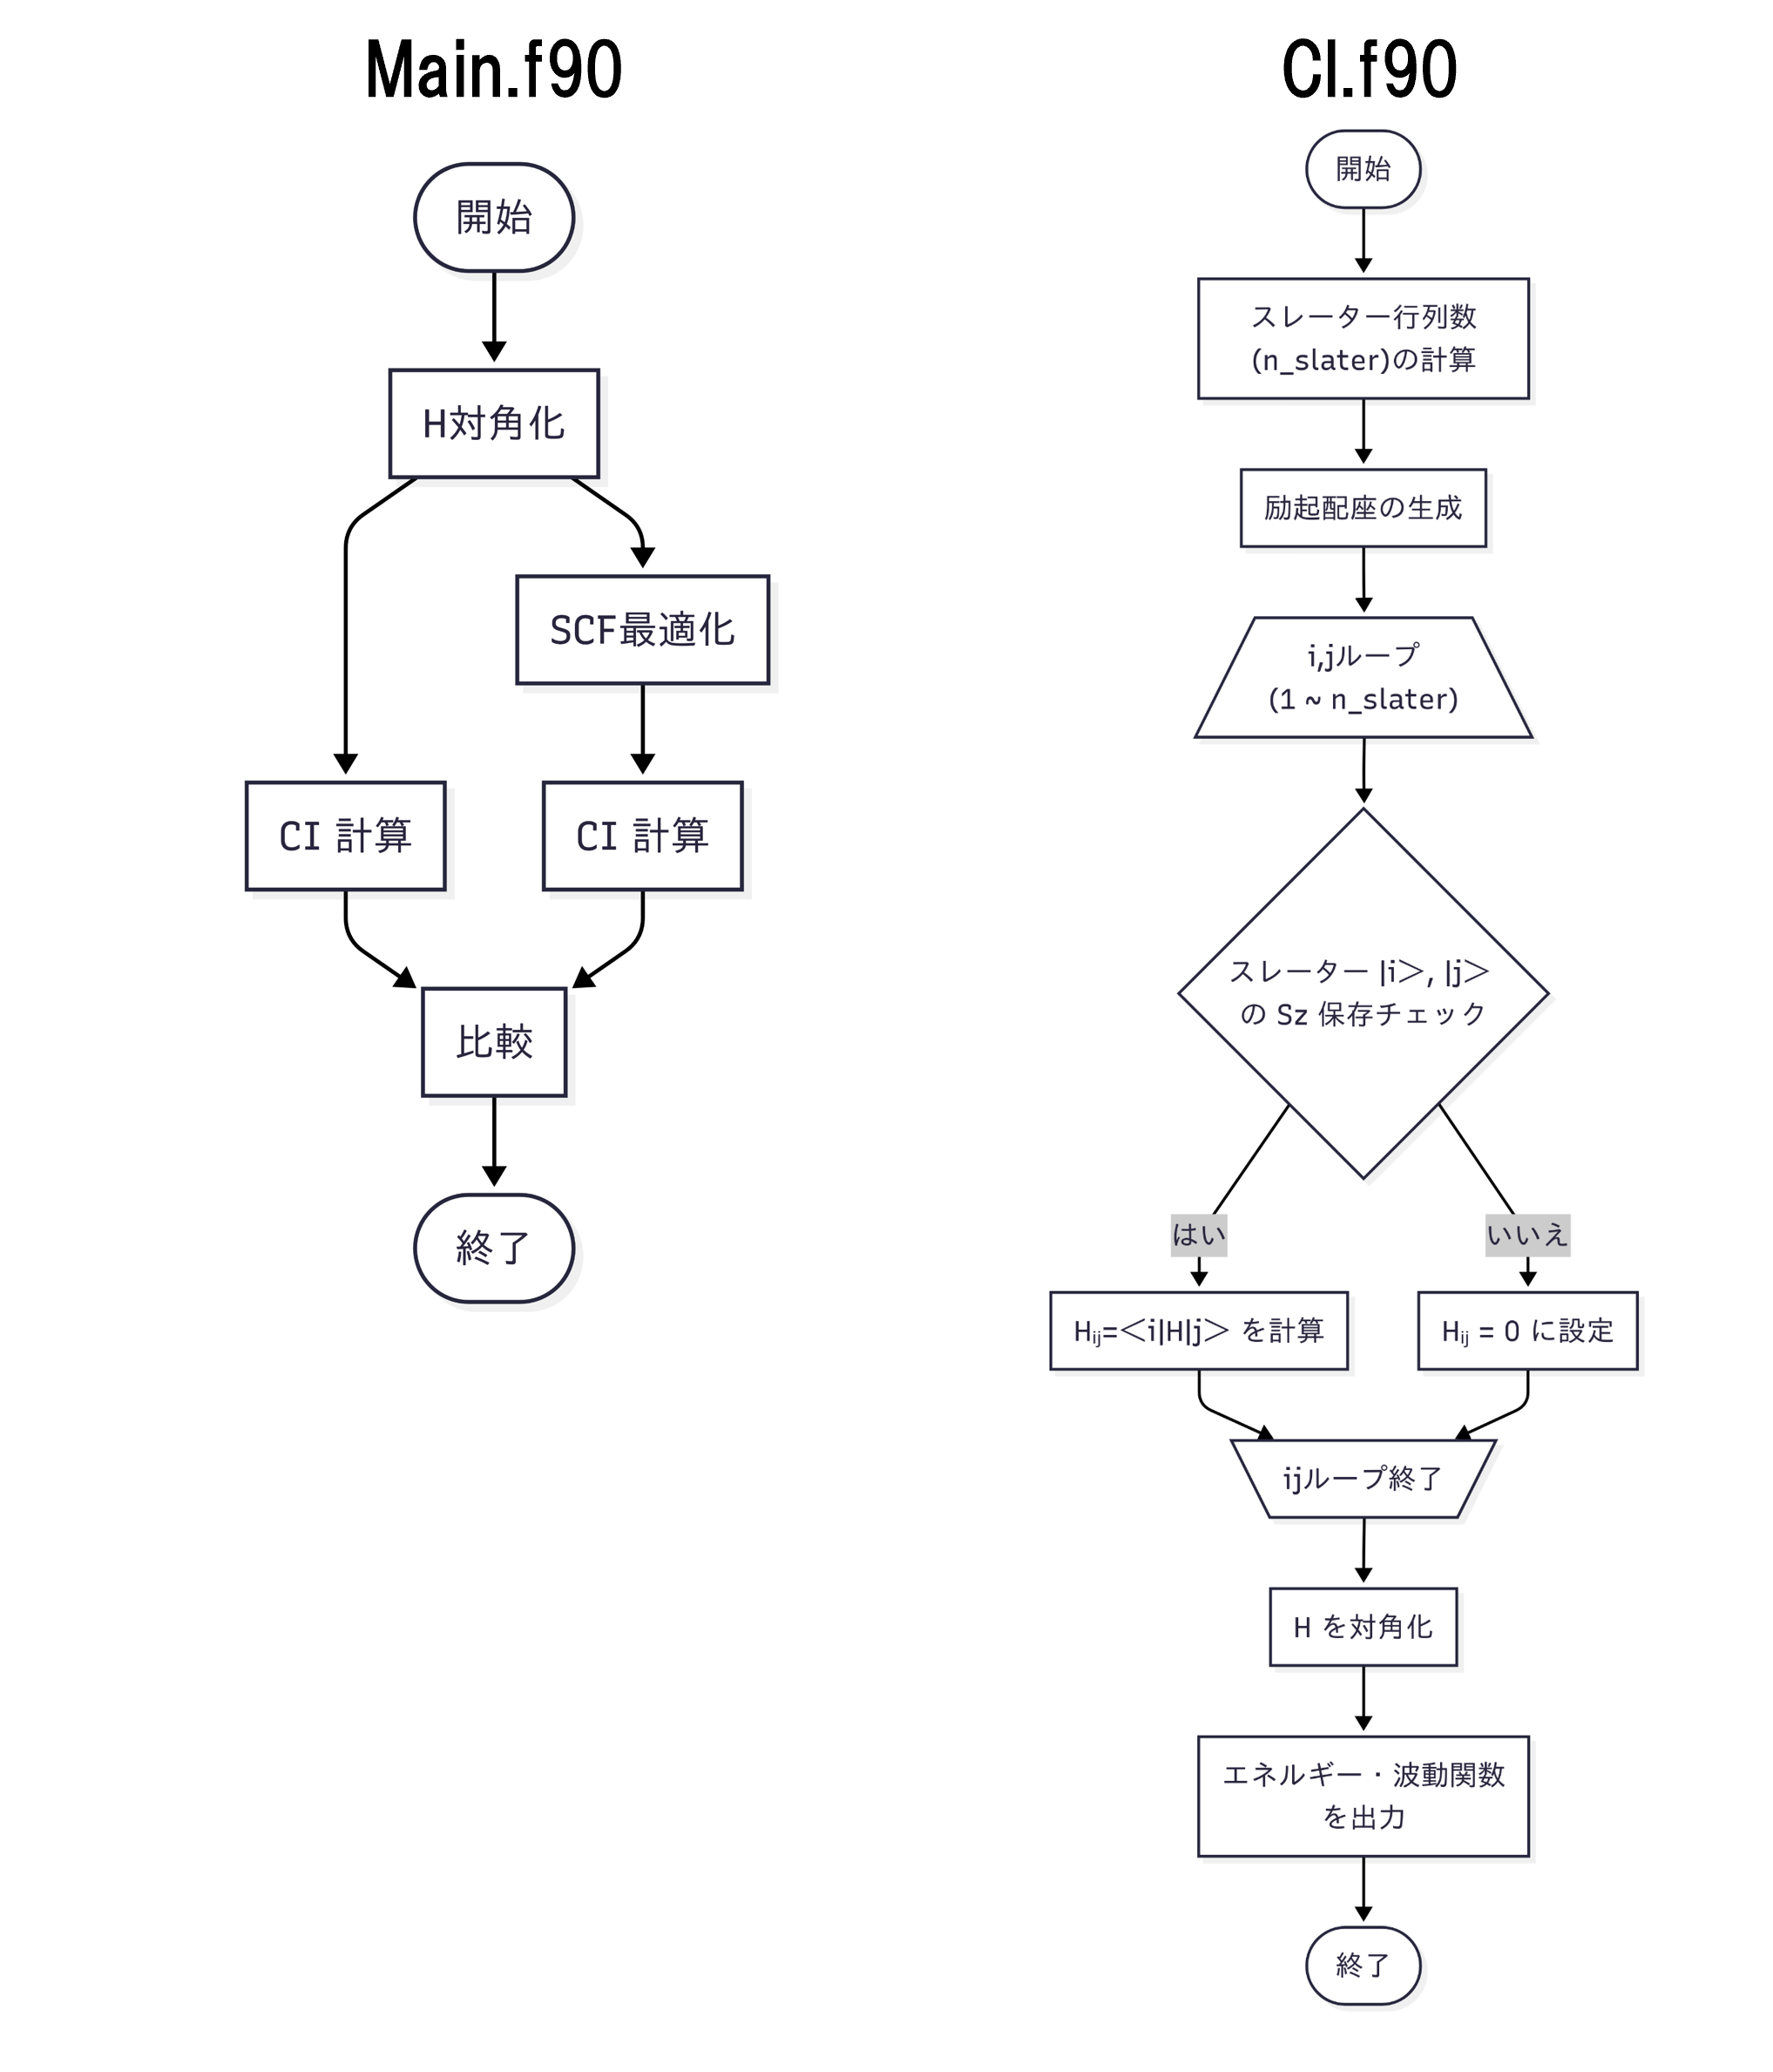
\includegraphics[width=0.8\linewidth]{imeges/フローチャート.png}
    \end{center}  
  \end{columns}
一電子系H演算子の波動関数とSCF最適化されたF演算子の波動関数のそれぞれでCI計算を行い,比較するプログラムを作成した.
  \end{frame}  

 

\begin{frame}{第3章 結果の考察}
  今回は100nmサイズのInSb量子ドットに閉じ込めた二電子系を対象に,
  Singlet状態とTriplet状態で,SCFCIと非SCFCIの結果をを比較した.

  特に次二項目についえ整理した..
  \begin{itemize}
    \item 多電子波動関数の比較
    \item エネルギーのω依存性
  \end{itemize}
\end{frame}  

\begin{frame}{3.1 多電子波動関数の比較}
  \textbf{Singlet(1-2配座) $\omega=15[a.u.]$}
  \begin{columns}
  \column{1.0\textwidth} 
  \begin{center}
      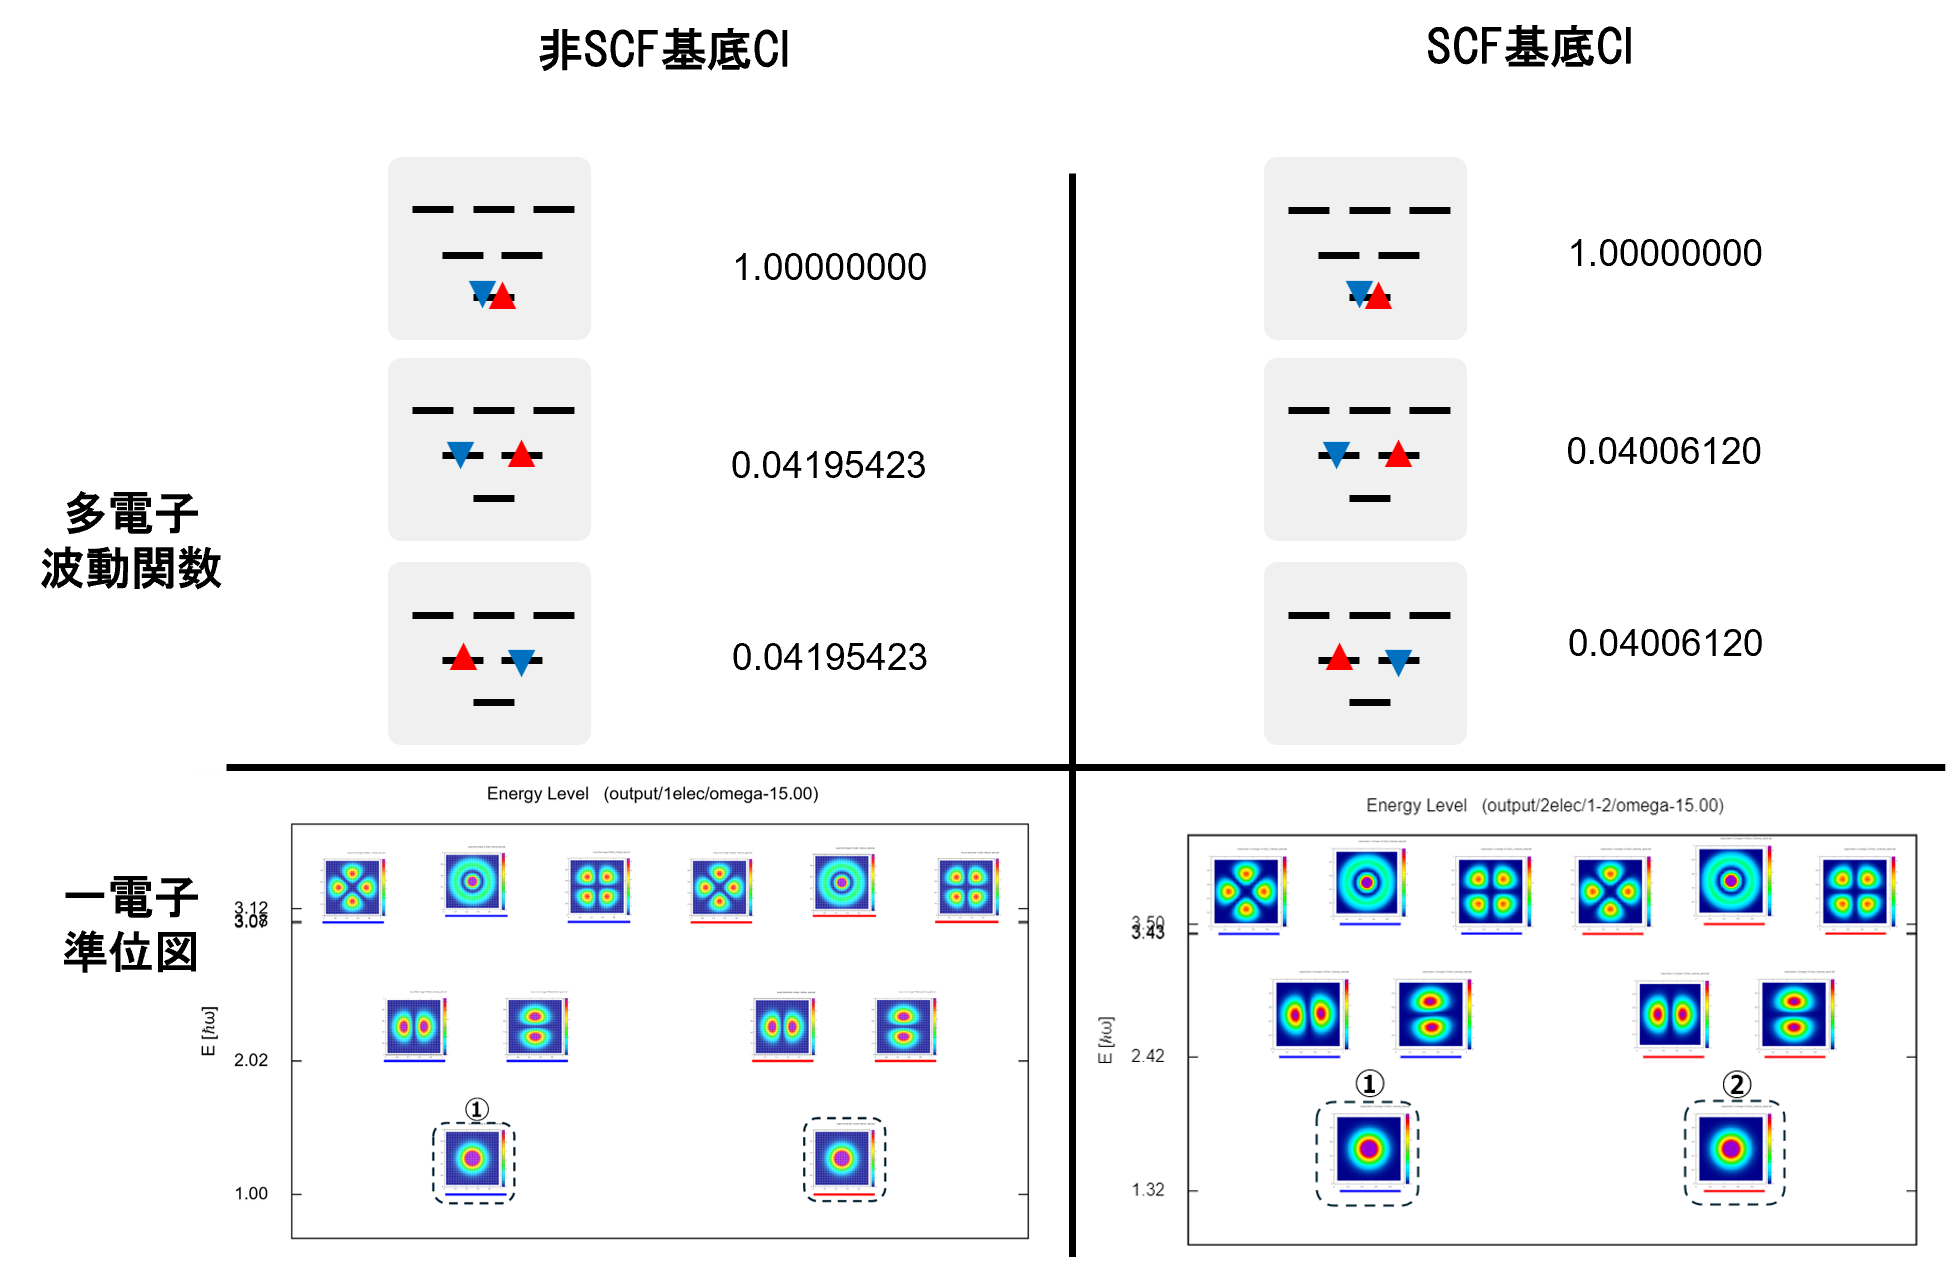
\includegraphics[width=1.0\linewidth]{imeges/1-2/波動関数.png}
  \end{center}
\end{columns}
\end{frame}  

\begin{frame}{}
  \textbf{Triplet(1-3配座) $\omega=15[a.u.]$}
  \begin{columns}
  \column{1.0\textwidth} 
  \begin{center}
      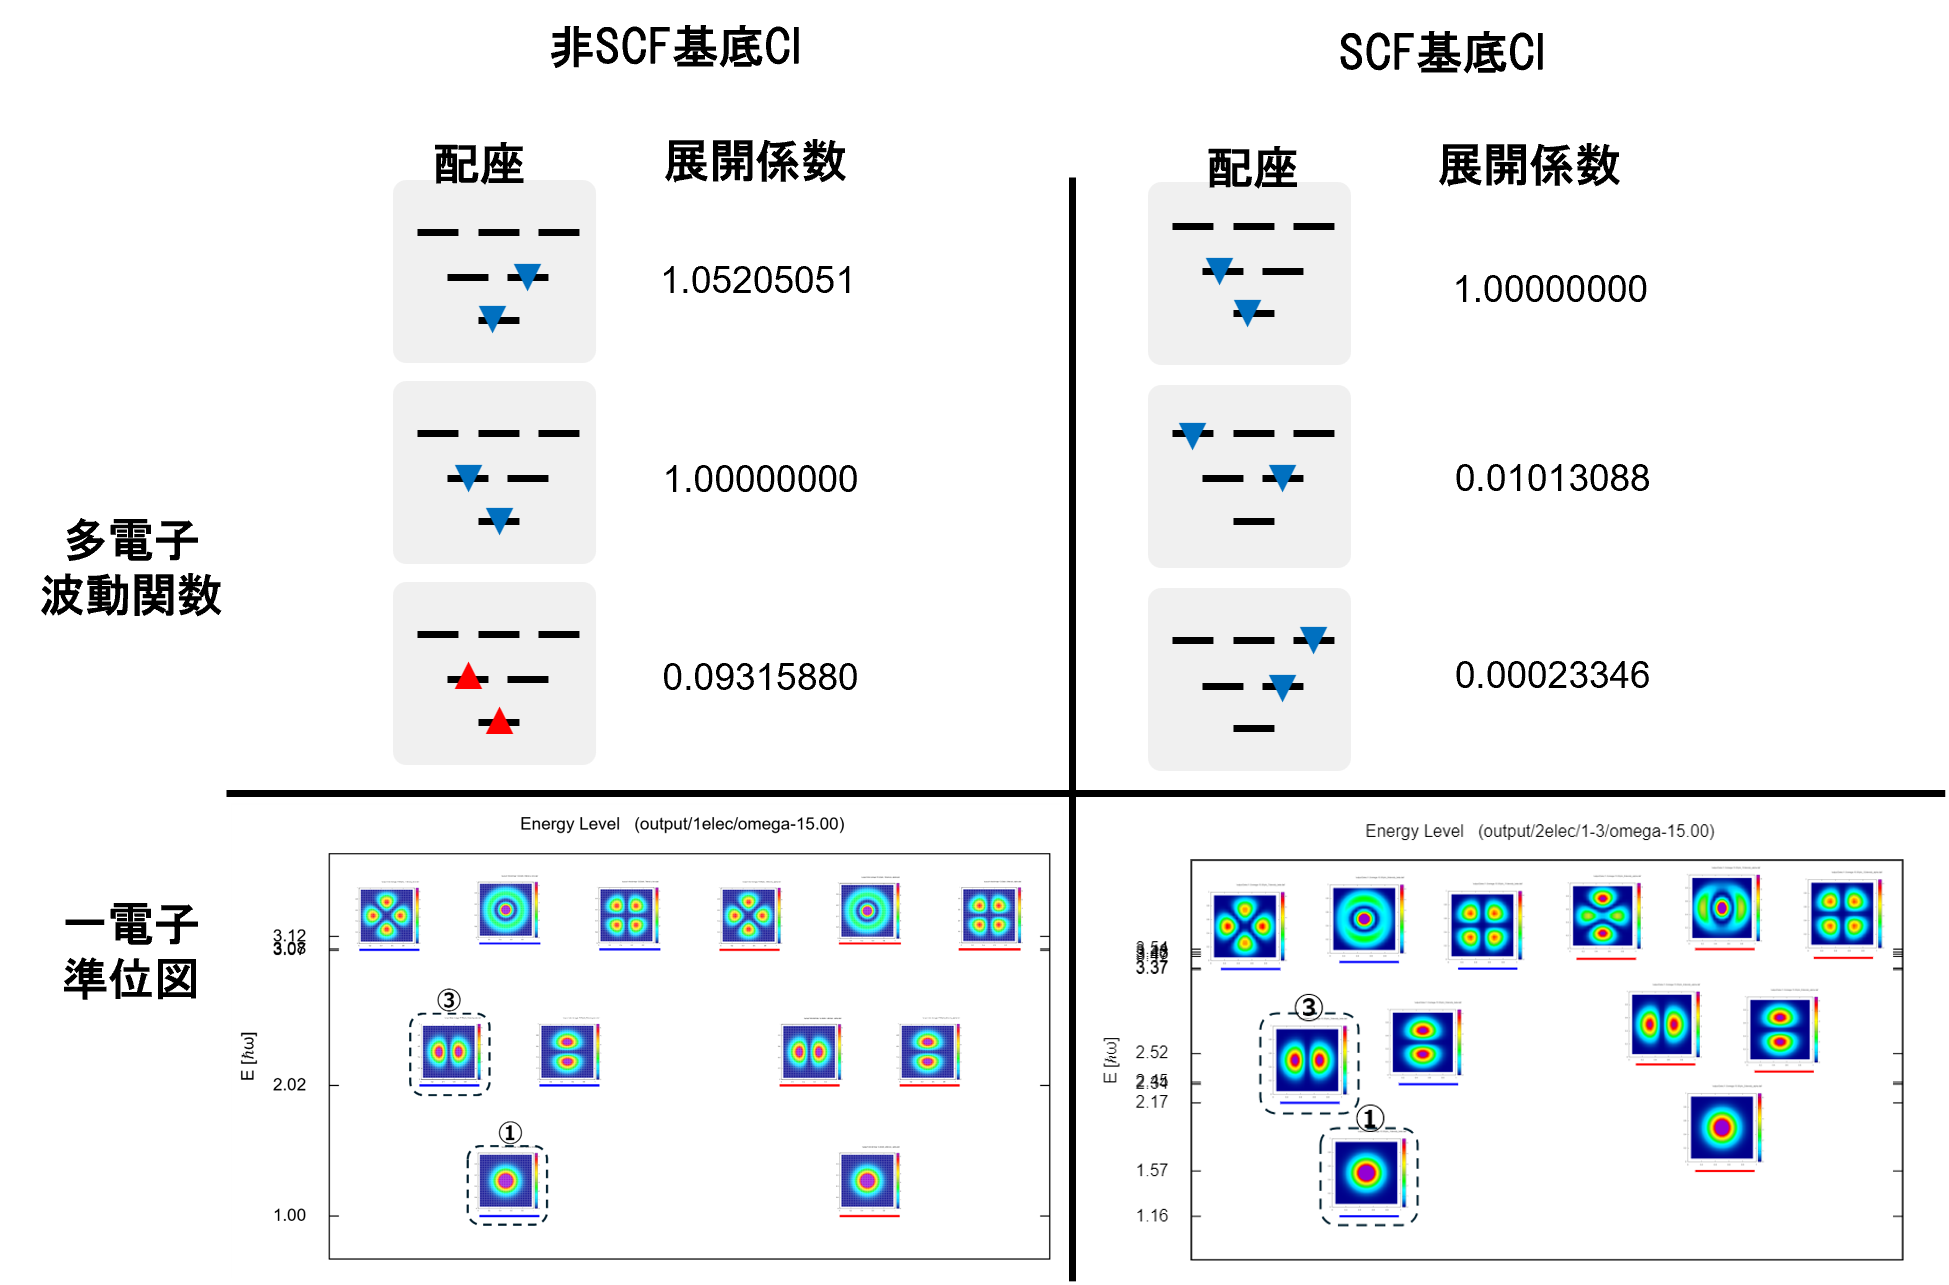
\includegraphics[width=1.0\linewidth]{imeges/1-3/波動関数.png}
  \end{center}
\end{columns}
非SCF基底の多電子波動関数は縮退軌道が混成しているので,jzユニタリ変換を施す必要がある.
\end{frame}  

\begin{frame}{3.2 多電子波動関数の比較}
  \textbf{Singlet(1-2配座)}
  \begin{columns}
  \column{1.0\textwidth}
    \begin{center}
        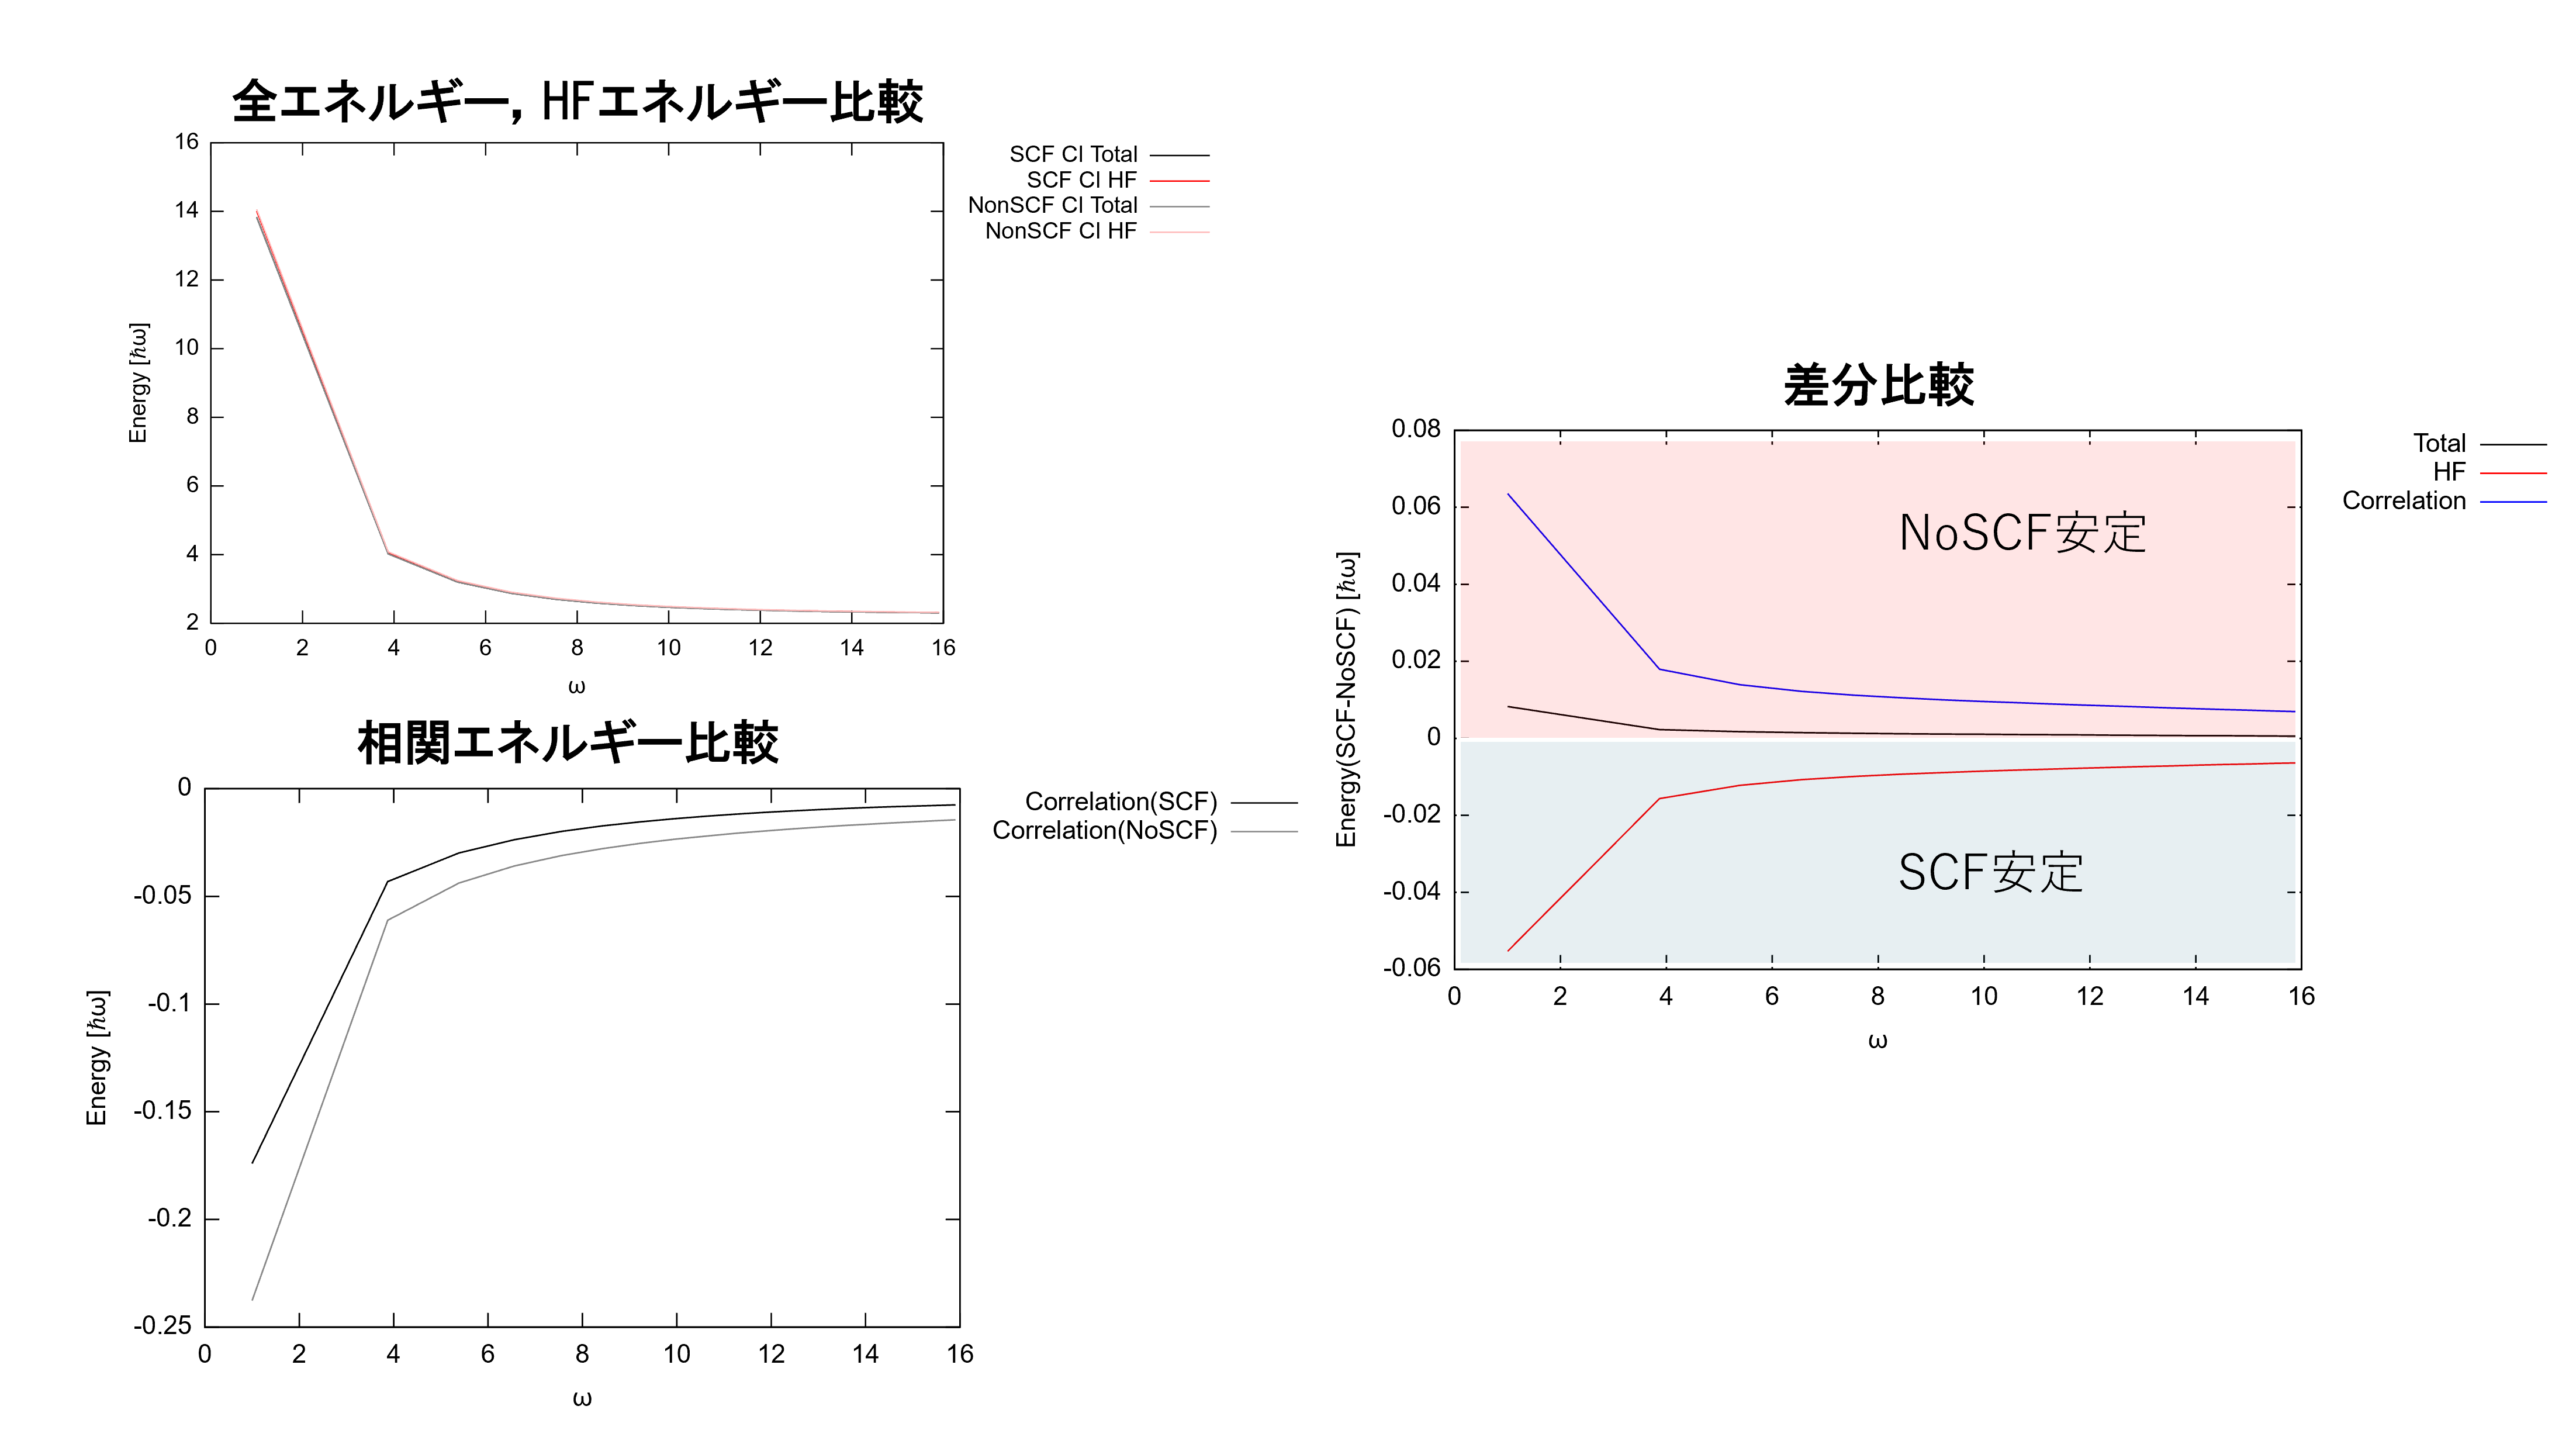
\includegraphics[width=1.0\linewidth]{imeges/1-2/画像5.png}
    \end{center}
  \end{columns} 
相関による非SCFCIの安定について,今回のsinglet系の計算では一電子軌道の対称性はどちらも保たれているので,対称性が原因ではないと考えられる.
\end{frame}  

\begin{frame}{}
  \textbf{Triplet(1-3配座)}
  \begin{columns}
  \column{1.0\textwidth}
    \begin{center}
        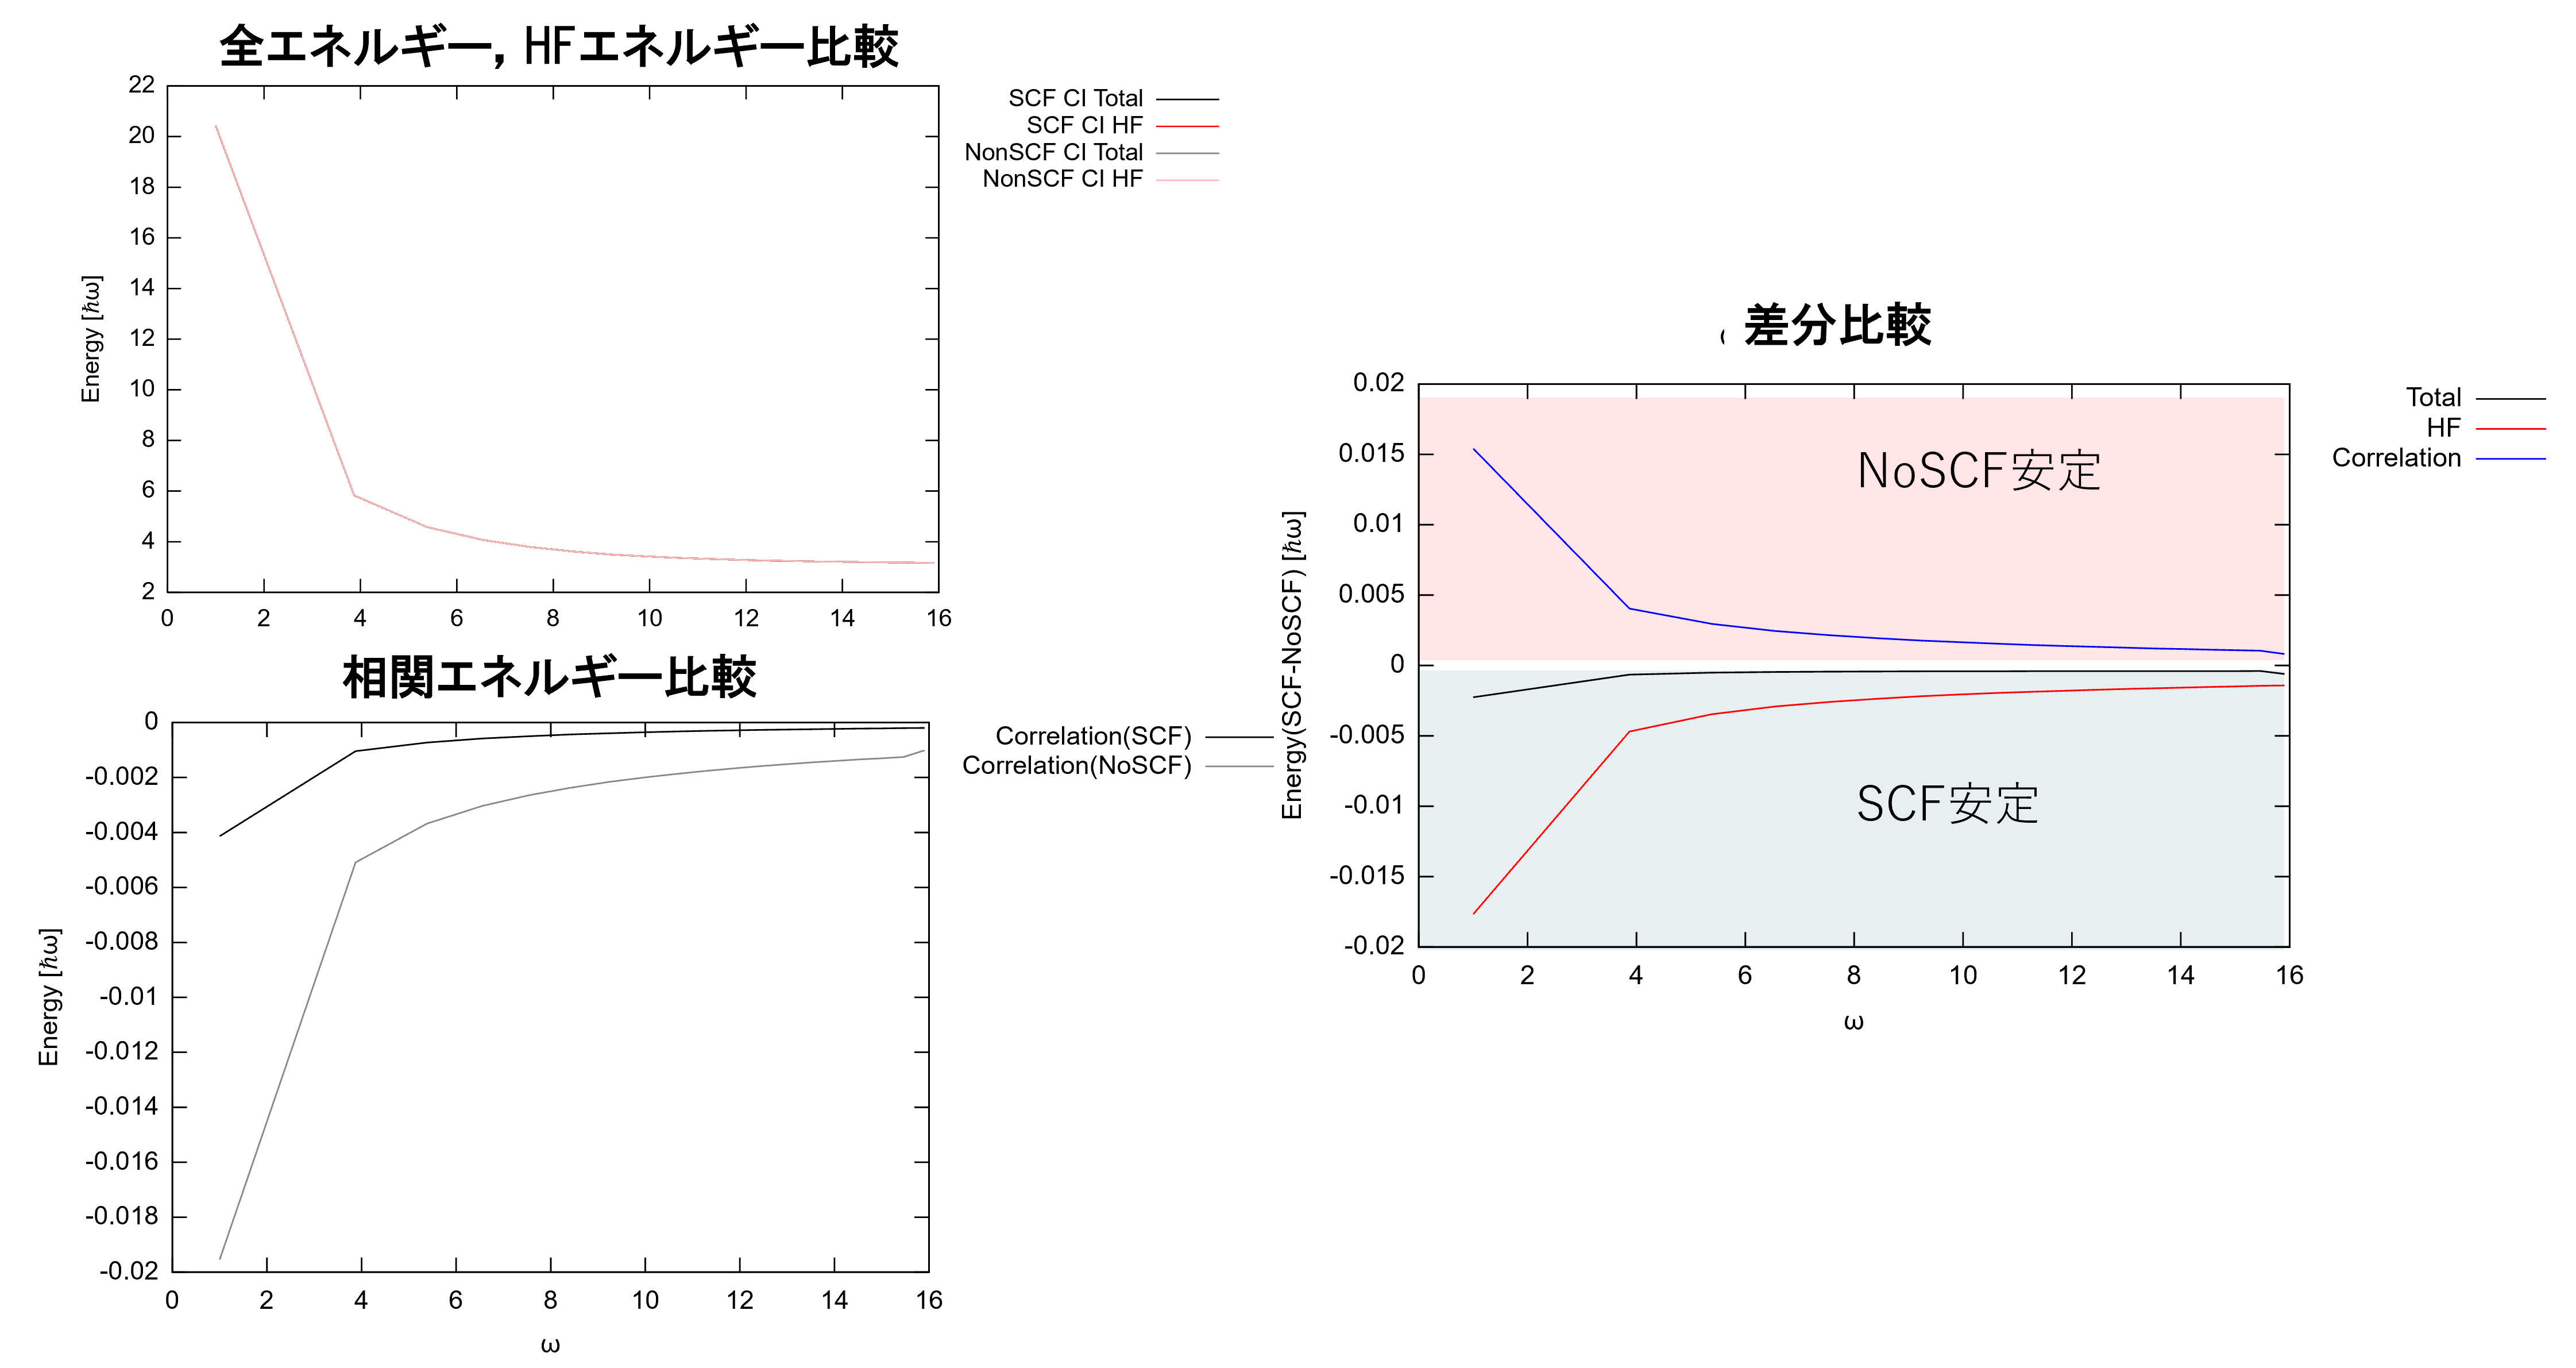
\includegraphics[width=1.0\linewidth]{imeges/1-3/データエネルギー.png}
    \end{center}
  \end{columns}
    相関エネルギーによる安定化が上回り,SCFCIのほうのエネルギーが安定した. 
\end{frame}  


\end{document}